\begin{problem}{1}
    Find $(-8 -8\sqrt{3}i)^{1/4}$, express the roots in rectangular coordinates, and exhibit them as the vertices of a certain square.
\end{problem}

\section*{Solución}


El número complejo $z$ esta dado por 

\begin{gather*}
    z = (-8 -8\sqrt{3}i)
\end{gather*}

Donde $\Re = -8$ y $\Im = -8 \sqrt{3}$. Expresando entonces en su forma polar, se debe calcular la norma 

\begin{gather*}
    |z|^2 = zz^{*} = (-8 - 8\sqrt{3}i)(-8 + 8\sqrt{3}i)\\
    |z|^2 = (-8)^2 - (8\sqrt{3}i)^2\\
    |z|^2 = 64 + (64(3)) = 4(64)\\
    |z| = 8\sqrt{4} = 16
\end{gather*}

y su argumento

\begin{gather*}
    \theta = \arctan\left(\frac{-8\sqrt{3}}{-8}\right)\\
    \theta = \arctan\left(\sqrt{3}\right) = \frac{\pi}{3}
\end{gather*}

Por tanto, expresando el número complejo en forma polar. 

\begin{gather*}
    z = 16e^{i\frac{\pi}{3}}\\
    z^{\frac{1}{4}} = \left( 16e^{i\frac{\pi}{3}}\right)^{\frac{1}{4}}
\end{gather*}

Implementando el teorema de De Moivre 

\begin{gather*}
    r^ne^{in\theta} = r^n\cos(n\theta) + i\sin(n\theta)\\
    z^{\frac{1}{4}} = 2 e^{i\frac{\pi}{3}\frac{1}{4}} = 2 \left[\cos\left(\frac{\pi/3 + 2n\pi}{4} \right) + i\sin\left(\frac{\pi/3 + 2n\pi}{4}\right)\right]
\end{gather*}

Entonces las raíces del número complejo serán:

\begin{gather*}
    z_1 = 2 \left[\cos\left(\frac{\pi}{12} \right) + i\sin\left(\frac{\pi}{12}\right)\right] = 2 \left[\frac{\sqrt{6} + \sqrt{2}}{4} + i \frac{\sqrt{6} - \sqrt{2}}{4} \right]\\
    z_2 = 2 \left[\cos\left(\frac{7\pi}{12} \right) + i\sin\left(\frac{7\pi}{12}\right)\right] = 2 \left[\frac{-\sqrt{6} + \sqrt{2}}{4} + i \frac{\sqrt{6} + \sqrt{2}}{4} \right]\\
    z_3 = 2 \left[\cos\left(\frac{13\pi}{12} \right) + i\sin\left(\frac{13\pi}{12}\right)\right]= 2 \left[-\frac{\sqrt{6} + \sqrt{2}}{4} + i \frac{-\sqrt{6} + \sqrt{2}}{4} \right]\\
    z_4 = 2 \left[\cos\left(\frac{19\pi}{12} \right) + i\sin\left(\frac{19\pi}{12}\right)\right] =  2 \left[\frac{\sqrt{6} - \sqrt{2}}{4} - i \frac{\sqrt{6} + \sqrt{2}}{4} \right]\\
\end{gather*}

Y entonces se demuestra que son los vertices de un cuadrado en el plano complejo 

\begin{figure}[h]
    \centering
    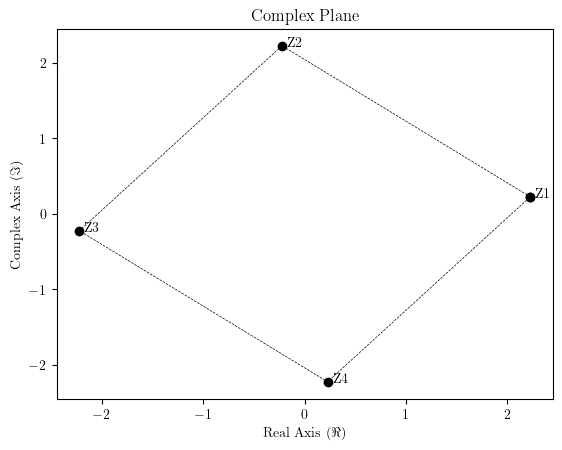
\includegraphics[scale = 1]{imgs/P1.png}
\end{figure}
